\documentclass[spanish,letterpaper,oneside]{article}

% Datos del documento
\def\documenttitle {Proporcionalidad directa e inversa en un lanzador}
\def\documentsubtitle {Temas selectos de matemáticas I}
\def\documentsubject {Actividad 4 · Resolución y análisis del modelo}
\def\documentauthor {Mtro. Martín Jonathan de la Cruz Muñoz}
\def\coursename {Temas selectos de matemáticas I}
\def\coursecode {PFM02}

% Identidad institucional
\def\universityname {Instituto de Investigación, Innovación y Estudios de Posgrado para la Educación del Estado de Nuevo León}
\def\universityfaculty {Maestría en Aprendizaje y Enseñanza de las Matemáticas}
\def\universitydepartment {Temas selectos de matemáticas I}
\def\universitydepartmentimage {img/iiiepe/marca-iiiepe.png}
\def\universitydepartmentimagecfg {height=1.75cm}
\def\universitylocation {Monterrey, Nuevo León}
\def\studentfullname {Mtro. Martín Jonathan de la Cruz Muñoz}
\def\studentid {00874}
\def\studentemail {martin.delacruz@campus.iiiepe.edu.mx}
\def\programperiod {1er tetramestre, marzo--julio de 2026}
\def\programmodality {Modalidad presencial}
\def\programshort {MAEM}

\def\authortable {
  \begin{tabular}{ll}
    \textbf{Alumno:} & \studentfullname \\
    Matrícula: & \studentid \\
    Correo institucional: & \studentemail \\
    Unidad: & \coursename \\
    Programa: & \programshort \\
    Periodo: & \programperiod \\
    & \\
    \multicolumn{2}{l}{Fecha de realización: 13 de octubre de 2026} \\
    \multicolumn{2}{l}{\universitylocation}
  \end{tabular}
}

\input{template}

\usepackage{helvet}
\renewcommand{\familydefault}{\sfdefault}
\usepackage{array}
\usepackage{longtable}
\usepackage{pdflscape}
\usepackage{tikz}
\usepackage[most]{tcolorbox}
\usetikzlibrary{arrows.meta,positioning,calc,fit,backgrounds}

\definecolor{iiiepeNavy}{HTML}{163B5C}
\definecolor{iiiepeBlue}{HTML}{1F6F9F}
\definecolor{iiiepeAqua}{HTML}{20B7A8}
\definecolor{iiiepeOrange}{HTML}{F28C28}
\definecolor{iiiepePaper}{HTML}{F6F8F7}
\definecolor{iiiepeInk}{HTML}{1E2A32}
\def\portraittitlecolor {iiiepeNavy}
\setcitestyle{authoryear,open={(},close={)}}

\newcommand{\insertcoverwatermark}{%
  \AddToShipoutPictureBG*{%
    \begin{tikzpicture}[remember picture,overlay]
      \node[opacity=.09,inner sep=0pt] at (current page.center)
      {\includegraphics[width=.58\paperwidth]{img/iiiepe/logo-puntos.png}};
    \end{tikzpicture}%
  }%
}

\newtcolorbox{reportelecturabox}[1][]{%
  enhanced,breakable,
  colback=iiiepePaper,colframe=iiiepeNavy,
  boxrule=1pt,leftrule=4pt,arc=2pt,
  left=8pt,right=8pt,top=6pt,bottom=6pt,
  before skip=6pt,after skip=10pt,
  fonttitle=\bfseries\color{white},coltitle=white,
  colbacktitle=iiiepeNavy,
  attach boxed title to top left={xshift=8pt,yshift=-2pt},
  boxed title style={colback=iiiepeNavy,colframe=iiiepeNavy,arc=1pt},
  title={Reporte de lectura},#1}

\newtcolorbox{fichalecturabox}[1][]{%
  enhanced,breakable,
  colback=iiiepeAqua!7,colframe=iiiepeAqua!70!iiiepeNavy,
  boxrule=.6pt,arc=1pt,
  left=7pt,right=7pt,top=4pt,bottom=4pt,
  fontupper=\small,before upper={\setstretch{1.0}},
  fonttitle=\bfseries\color{iiiepeNavy},coltitle=iiiepeNavy,
  colbacktitle=iiiepeAqua!7,
  title={Ficha de la lectura},#1}



\usepackage{tabularx,colortbl,pgfplots,enumitem,needspace}\pgfplotsset{compat=1.18}\definecolor{iiiepePale}{HTML}{EEF5F8}
\setlength{\parskip}{5pt}\setlength{\parindent}{0pt}
\begin{document}\insertcoverwatermark\templatePortrait\templatePagecfg\templateFinalcfg\fancyfoot{}\fancyfoot[L]{\scriptsize IIIEPE · MAEM}\fancyfoot[C]{\scriptsize\thepage}\fancyfoot[R]{\scriptsize Actividad 4}\setstretch{1.3}\raggedbottom
\section{Proporcionalidad y control de variables}
Una relación directa tiene la forma $y=kx$: el cociente $y/x$ permanece constante. Una relación inversa tiene la forma $y=k/x$: el producto $xy$ permanece constante. Observar que una cantidad aumenta mientras otra disminuye es insuficiente para afirmar proporcionalidad inversa; es necesario comprobar el producto y justificar las condiciones del modelo.
\section{Fase 1 · Saberes de nuestra comunidad}
Una piedra y una pluma no necesariamente alcanzan la misma distancia con un lanzamiento aparentemente semejante. La aceleración depende de $F/m$, pero la resistencia del aire, la forma, la superficie y el tiempo de aplicación de la fuerza también intervienen. Si se duplica la masa, no es posible determinar una distancia exacta solo con la frase ``misma fuerza''. En un modelo de energía constante, ángulo fijo, igual altura y resistencia despreciable, el alcance sí puede ser inversamente proporcional a la masa.
Un ejemplo exacto de proporcionalidad inversa es el tiempo y la velocidad para un recorrido fijo: $t=D/v$. El supuesto de distancia constante es indispensable.
\section{Fases 2 y 3 · Indagación y diseño}
La hipótesis es que, con energía de lanzamiento comparable, el alcance disminuya al aumentar la masa. Comparar papel y canica confunde masa con resistencia aerodinámica; propondría proyectiles de espuma del mismo tamaño con pequeñas diferencias de masa. El boceto debe incluir base estable, brazo articulado, liga, soporte y tope que fije el retroceso en 5 cm. Solo usaría proyectiles blandos, una zona delimitada y un lanzamiento dirigido lejos de personas.
\begin{center}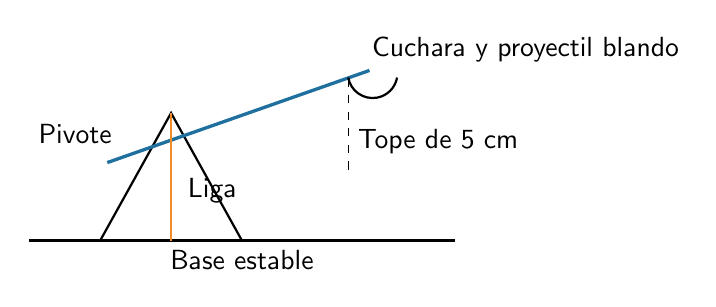
\begin{tikzpicture}[scale=.9]
\draw[very thick] (0,0)--(6,0);\draw[thick] (1,0)--(2,1.8)--(3,0);\draw[very thick,iiiepeBlue] (1.1,1.1)--(4.8,2.4);\draw[iiiepeOrange,thick] (2,1.8)--(2,0);\draw[thick] (4.5,2.3) arc(190:350:.35);\node[below] at (3,0){Base estable};\node[left] at (1.3,1.5){Pivote};\node[right] at (4.7,2.7){Cuchara y proyectil blando};\node[right] at (2.1,.7){Liga};\draw[dashed] (4.5,1)--(4.5,2.3);\node[right] at (4.5,1.4){Tope de 5 cm};
\end{tikzpicture}\end{center}
Un problema técnico previsible es que la base se desplace y altere el ángulo. Lo resolvería fijándola a una tabla y documentando cualquier cambio. El boceto representa una alternativa de ajuste del diseño; las pruebas disponibles constituyen la referencia de aplicación y no se les atribuye este cambio específico.
\section{Fase 4 · Tabla, gráfica y modelo}
La ficha exige mediciones físicas. La siguiente tabla es un \textbf{ejemplo simulado para explicar el procedimiento}; se distingue de las mediciones y pruebas reales disponibles, cuya referencia en este reporte es cualitativa. Las masas numéricas permiten graficar una variable cuantitativa; ``ligero, medio y pesado'' por sí solos no permiten verificar $md=k$.


{\small\setstretch{1.1}\renewcommand{\arraystretch}{1.25}
\begin{longtable}{|>{\raggedright\arraybackslash}p{\dimexpr0.25\linewidth-2\tabcolsep-2\arrayrulewidth\relax}|>{\raggedright\arraybackslash}p{\dimexpr0.25\linewidth-2\tabcolsep-2\arrayrulewidth\relax}|>{\raggedright\arraybackslash}p{\dimexpr0.25\linewidth-2\tabcolsep-2\arrayrulewidth\relax}|>{\raggedright\arraybackslash}p{\dimexpr0.25\linewidth-2\tabcolsep-2\arrayrulewidth\relax}|}\hline
\rowcolor{iiiepePale} \textbf{Masa (g)} & \textbf{Tiro 1 (cm)} & \textbf{Tiro 2 (cm)} & \textbf{Promedio (cm)} \\\hline
\endfirsthead
\hline
\rowcolor{iiiepePale} \textbf{Masa (g)} & \textbf{Tiro 1 (cm)} & \textbf{Tiro 2 (cm)} & \textbf{Promedio (cm)} \\\hline
\endhead
2 & 118 & 122 & 120 \\\hline
4 & 58 & 62 & 60 \\\hline
6 & 38 & 42 & 40 \\\hline
\end{longtable}}


En estos datos construidos, $md=240$ g·cm y $d=240/m$ cm. La constante no es una fuerza: sus unidades son masa por distancia. Bajo un modelo ideal de energía elástica $E$, $v^2=2E/m$ y $R=v^2\sin(2\theta)/g$; así $R=(2E\sin(2\theta)/g)/m$. El ajuste experimental debe comprobarse y no imponerse a los datos.
\begin{center}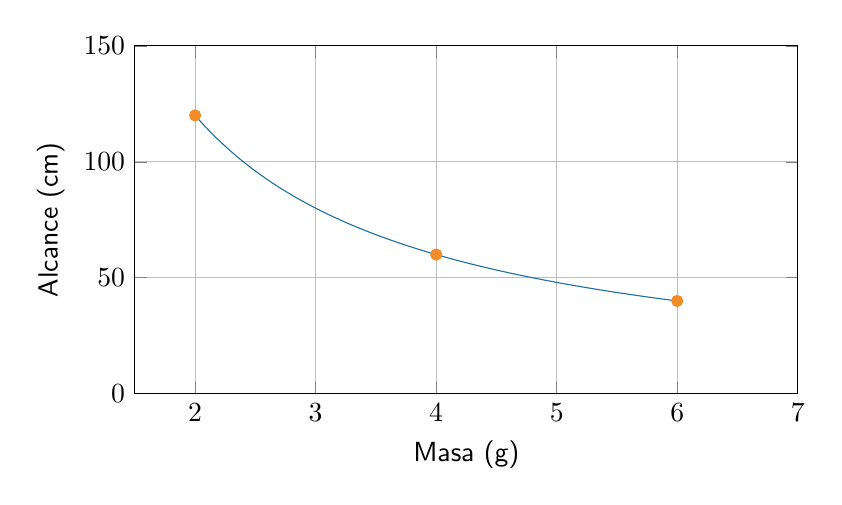
\begin{tikzpicture}\begin{axis}[width=10cm,height=6cm,xlabel={Masa (g)},ylabel={Alcance (cm)},xmin=1.5,xmax=7,ymin=0,ymax=150,grid=major]
\addplot[iiiepeBlue,domain=2:6,samples=70]{240/x};\addplot[only marks,iiiepeOrange] coordinates {(2,120)(4,60)(6,40)};
\end{axis}\end{tikzpicture}\end{center}
Para una masa de 10 kg no extrapolaría una catapulta escolar. El modelo numérico daría $240/10000=0.024$ cm, pero está fuera del intervalo observado y de la capacidad del dispositivo. Obtener una cifra no demuestra validez física.
\subsection*{Problemas de aplicación}
El camión recorre $60(4)=240$ km. Para completar el mismo recorrido en 3 horas, $v=240/3=80$ km/h, dentro del modelo de velocidad constante. Para el trabajo divisible y rendimiento individual constante, $4(45)=180$ persona-minutos; seis cadetes tardarían $180/6=30$ minutos. La coordinación y tareas indivisibles pueden modificar el resultado real.
\section{Diseño experimental reproducible}
La variable modificada será la masa medida en gramos; la respuesta será el alcance horizontal en centímetros. Se mantendrán base, ángulo, retroceso, punto de referencia y proyectiles de geometría comparable. Antes de registrar, se verificará que el instrumento de masa distingue las diferencias entre proyectiles. Dos tiros son el mínimo del recurso; propongo cinco para examinar variabilidad con mayor claridad, sin afirmar que ese número garantice validez estadística.
Para cada masa se calcularán promedio y rango. Se compararán tanto $md$ como sus variaciones: una tendencia descendente puede corresponder a otras funciones. Si las discrepancias superan la incertidumbre razonable del registro, se rechazará la proporcionalidad inversa simple o se limitará su intervalo. La decisión se basará en las observaciones, no en completar la frase de la ficha con una respuesta esperada.
\subsection{Lectura cualitativa de las mediciones y pruebas}
Se cuenta con mediciones y pruebas del dispositivo. La referencia a ellas se mantiene cualitativa y atiende a cuatro dimensiones: estabilidad de las condiciones de lanzamiento, consistencia del registro, relación entre predicción y observación y razones para revisar el diseño. La existencia de pruebas permite situar la reflexión en una experiencia de aplicación; sus resultados específicos no se sustituyen por los números del ejemplo didáctico.
El criterio de interpretación es contrastar el comportamiento registrado con los supuestos del modelo. Una conclusión responsable debe explicar qué condiciones se mantuvieron y qué límite tiene la comparación. En esta versión se desarrolla ese criterio y la resolución matemática; no se transcriben las series numéricas de las mediciones disponibles.
\section{Secuencia de aplicación y evaluación}
Contrastar proporcionalidad mediante registros y condiciones controladas. La duración propuesta es de 100 minutos, ajustable al diagnóstico y a los recursos. Esta planeación sigue la progresión de los recursos institucionales (IIIEPE, 2026); los tiempos y apoyos son decisiones de codiseño, no datos de una aplicación ya realizada.

{\small\setstretch{1.1}\renewcommand{\arraystretch}{1.25}
\begin{longtable}{|>{\raggedright\arraybackslash}p{\dimexpr0.23\linewidth-2\tabcolsep-2\arrayrulewidth\relax}|>{\raggedright\arraybackslash}p{\dimexpr0.49\linewidth-2\tabcolsep-2\arrayrulewidth\relax}|>{\raggedright\arraybackslash}p{\dimexpr0.28\linewidth-2\tabcolsep-2\arrayrulewidth\relax}|}\hline
\rowcolor{iiiepePale} \textbf{Fase y tiempo} & \textbf{Actividad y mediación} & \textbf{Evidencia} \\\hline
\endfirsthead
\hline
\rowcolor{iiiepePale} \textbf{Fase y tiempo} & \textbf{Actividad y mediación} & \textbf{Evidencia} \\\hline
\endhead
1. Reto y saberes (12 min) & Anticipar la relación entre masa y alcance y declarar una hipótesis. & Predicción individual y pregunta. \\\hline
2. Plan de indagación (18 min) & Definir variables, escala, controles y condiciones de seguridad. & Plan explicado y criterios. \\\hline
3. Construcción y análisis (35 min) & Construir o revisar el prototipo y registrar tiros reales. & Registro o procedimiento trazable. \\\hline
4. Comunicación y aplicación (20 min) & Representar datos y comprobar producto o cociente dentro del intervalo. & Argumento con comprobación. \\\hline
5. Metacognición (15 min) & Aceptar, limitar o rechazar el modelo explicando la evidencia. & Versión revisada y justificación. \\\hline
\end{longtable}}
\subsection{Criterios observables y retroalimentación}

{\small\setstretch{1.1}\renewcommand{\arraystretch}{1.25}
\begin{longtable}{|>{\raggedright\arraybackslash}p{\dimexpr0.22\linewidth-2\tabcolsep-2\arrayrulewidth\relax}|>{\raggedright\arraybackslash}p{\dimexpr0.4\linewidth-2\tabcolsep-2\arrayrulewidth\relax}|>{\raggedright\arraybackslash}p{\dimexpr0.38\linewidth-2\tabcolsep-2\arrayrulewidth\relax}|}\hline
\rowcolor{iiiepePale} \textbf{Criterio} & \textbf{Evidencia de logro} & \textbf{Acción si necesita apoyo} \\\hline
\endfirsthead
\hline
\rowcolor{iiiepePale} \textbf{Criterio} & \textbf{Evidencia de logro} & \textbf{Acción si necesita apoyo} \\\hline
\endhead
Variables & Fija retroceso, ángulo y origen y modifica masa medida. & Revisar qué condición cambió entre tiros. \\\hline
Registro & Conserva todas las observaciones y distingue datos simulados. & Separar tabla de ensayo y tabla real; revisar unidades. \\\hline
Modelo & Compara productos o cocientes y muestra gráfica cuantitativa. & No aceptar relación inversa solo por una tendencia descendente. \\\hline
Conclusión & Delimita intervalo y reconoce variación o incertidumbre. & Pedir un dato que contradiga o limite la hipótesis. \\\hline
\end{longtable}}
El instrumento es una propuesta docente. Cada criterio se registra como logrado con autonomía, logrado con apoyo o aún no demostrado; no se asigna una calificación observada sin aplicar la actividad. En la coevaluación, un compañero verifica un criterio y formula una pregunta; en la autoevaluación, el estudiante explica una corrección; el docente contrasta ambas evidencias y decide el siguiente apoyo.\subsection{Participación y apoyos}
La inclusión se concreta en alternativas de representación y de acceso; el pensamiento crítico, en justificar y contrastar. Los roles de cálculo, registro y explicación se rotan para que todos produzcan una evidencia individual. Quien necesita apoyo dispone de un ejemplo parcial y preguntas graduadas; quien ya domina el procedimiento analiza un contraejemplo o cambia una condición. Estas acciones deben observarse durante la aplicación para valorar su funcionamiento.

\section{Fase 5 · Metacognición y reflexión pedagógica}
Para alcanzar la mitad de distancia con la misma masa, reduciría la energía y calibraría progresivamente el estiramiento. No afirmaría que basta reducirlo a la mitad: con una liga ideal y geometría constante, $E\propto s^2$ y el estiramiento aproximado sería $s/\sqrt2$. Tablas y gráficas permiten comparar hipótesis con mediciones, estimar dispersión y decidir el siguiente ajuste.
Rediseñaría la sesión para distinguir hipótesis, simulación y observación. En mantenimiento y mecatrónica esta distinción es habitual al calibrar equipos; en una enseñanza humanista se convierte además en una oportunidad para argumentar sin penalizar el dato inesperado. Rotaría los roles de medición, registro y diseño, y valoraría el control de variables, la explicación matemática y la revisión del prototipo.

\needspace{5\baselineskip}\section*{Referencias}
{\setstretch{1.15}\setlength{\parskip}{6pt}
\par\hangindent=1.27cm\hangafter=1  IIIEPE. (2026). \textit{Recurso sesión 4: Relaciones de proporcionalidad}. EVA posgrado.
\par\hangindent=1.27cm\hangafter=1  Secretaría de Educación Pública. (2024). \textit{Programa de estudio para la educación secundaria: Programa sintético de la Fase 6}. SEP.
}

\end{document}
